% !TEX root = ../00_thesis.tex

\section{System Model and Scheduling Problem}
\label{sec:model}

\fakepar{Nodes}
We denote by \nodeset the set of \emph{nodes} in the system.
Nodes implement distributed applications, composed of multiple tasks to execute and  messages to exchange.
A node is considered capable of performing one task execution and one message transmission simultaneously; this is supported by state-of-the-art wireless \cps platforms featuring two cores, such as the NXP LPC541XX~\cite{nxpLPC541XX}, VF3xxR~\cite{nxpVF3xxR}, or more generally any platform following the Dual-Processor Platform concept~(\cref{sec:dpp}).

\fakepar{Applications}
We denote by \appset the set of \emph{applications} in the system.
Each distributed application is composed of \emph{tasks} and \emph{messages} connected by precedence constraints described by a directed acyclic graph, where vertices and edges represent tasks and messages, respectively. We denote by \app.\predG the \emph{precedence graph} of application \app~(\cref{fig:precedence_graph}).
Each application executes at a periodic interval $\app.p$, called the \emph{period}.
An application execution is completed when all tasks in \predG have been executed.
All tasks and messages in \app.\predG share the same period, $\app.p$.
Applications are subject to real-time constraints: The application \emph{relative deadline}, denoted by $\app.d$ represents the maximum tolerable \emph{end-to-end delay} to complete the execution. The deadline is arbitrary (\ie it has no relation with the period $\app.p$).
Certain critical applications may require to keep the same schedule (\eg same task offsets) when switching between operation modes.
We call these \emph{persistent applications} and denote their set by \persappset; $\persappset \subset \appset$.
In summary, an application \app is characterized by

\pagebreak

\begin{align*}
\app \; = \; \{ \quad
	 \app.p
	\quad &\text{--\quad period} \\
	 \app.d
	\quad &\text{--\quad end-to-end deadline} \\
	 \app.\predG
	\quad &\text{--\quad precedence graph} \quad\quad \}
\end{align*}

\fakepar{Tasks}
We denote by \taskset the set of tasks.
A node executes at most one task at any point in time and we consider non-preemptive task scheduling.
Each task $\tau$ is mapped to a given node $\tau.map$, on which it executes within a WCET (worst-case execution time) $\tau.e$.
The \emph{task offset} $\tau.o$ represents the start of the task execution, relative to the beginning of the application execution.
A task can have an arbitrary number of preceding messages, \ie messages that must be received before the task can start. $\tau.prec$ denotes the set of preceding message \ids.
Within one application, each task is unique; however, the same task may belong to multiple applications (\eg the same sensing task may source different feedback loops). If so, we consider that these applications have the same period.
In summary, a task $\tau$ is characterized by
\begin{align*}
\tau \; = \; \{ \quad
	 \tau.o
	\quad &\text{--\quad offset} \\
	 \tau.\map
	\quad &\text{--\quad mapping} \\
	 \tau.e
	\quad &\text{--\quad WCET} \\
	 \tau.\prec
	\quad &\text{--\quad preceding message set} \\
	 \tau.p
	\quad &\text{--\quad period (equal to $\app.p$)} \quad \quad \}
\end{align*}

\fakepar{Messages}
We denote by \messageset the set of messages.
Every message $m$ has at least one preceding task, \ie a task that needs to finish before the message can be transmitted. The set of preceding task \ids is denoted by $m.prec$.
% All preceding tasks must be mapped to the same node.
The \emph{message offset} $m.o$, relative to the beginning of the application execution, represents the earliest time the message $m$ can be allocated to a round for transmission, \ie after all preceding tasks are completed.
The \emph{message deadline} $m.d$, relative to the message offset, represents the latest time when the message transmission must be completed, \ie the earliest offset of successor tasks.
All messages share the same maximal payload \Lmax.
Messages are not necessarily unique, \ie multiple edges of \app.\predG can be labeled with the same message $m$, which captures the case of multicast or broadcast~(\cref{fig:precedence_graph}).
If the same message belongs to multiple applications, we consider that these applications have the same period.
In summary, a message $m$ is characterized by
\begin{align*}
m \; = \; \{ \quad
	 m.o
	\quad &\text{--\quad offset} \\
	 m.d
	\quad &\text{--\quad deadline} \\
	 m.\prec
	\quad &\text{--\quad preceding task set} \\
	 m.p
	\quad &\text{--\quad period (equal to $\app.p$)} \quad \quad \}
\end{align*}


\begin{figure}
\centering
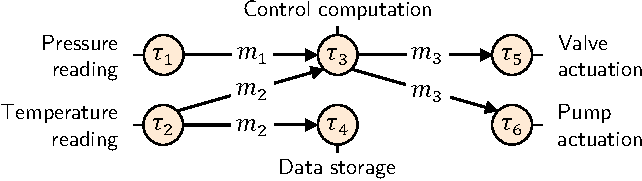
\includegraphics[scale=1]{precedence_graph}
\caption{An example application and its precedence graph \predG.
\capt{The execution starts with sensor readings -- either $\tau_1$ or $\tau_2$. After both have been received by the controller, actuation values are computed ($\tau_3$), multicast to the actuators ($m_3$), and applied ($\tau_5$ and $\tau_6$).
%All tasks must be completed before the application end-to-end deadline $\app.d$.
}}
\label{fig:precedence_graph}
\end{figure}

\pagebreak

\fakepar{Operation modes}
We denote by \modeset the set of operation modes (also simply called ``modes'').
These modes represent mutually exclusive phases of the system, \eg boostrapping, normal, and emergency modes; each having its own schedule.
Each mode has a unique \emph{priority} \modeany.\prio, used for scheduling purposes~(\cref{sec:multi_mode}).
A mode \modeany is characterized by
\begin{align*}
\modeany \; = \; \{ \quad
	 \appi\, , \;
	 \appj\, , \; \ldots
	\quad &\text{--\quad applications to execute}\\
	 \modeany.\prio
	\quad &\text{--\quad priority} \quad \}
\end{align*}
We write $\app \in \modeany$ to denote that \app is executing in mode \modeany.
When unambiguous, we use \modeany to denote the set of applications executing in mode \modeany.
The mode \emph{hyperperiod} \modeHyperperiod is the least common multiple of the mode's applications.
Possible transitions between modes at runtime are described with the \emph{mode graph} \modeGraph~(\cref{fig:modeGraph}). The mode graph is undirected; a transition from \modei to \modej implies that it is possible to transition from \modej to \modei as well.



\fakepar{Rounds}
The schedule of a mode \mode{} contains $R_{\mode{}}$ \emph{communication rounds} $r$.
Rounds are \emph{atomic}; that is, they cannot be interrupted. Therefore, the ordering of messages within one round does not matter.%
%
\footnote{\TTW could be extended to account for the relative ordering of messages in a round. In theory, this would allow to further reduce the achievable latency of applications at the cost of a more complex synthesis problem to solve.}
%
Each round $r$ is composed of \nslotsround slots (with a maximum of \nslotsmax), each allocated to a unique message $m$.
This results in a round length $\Tround = \Toffset + \nslotsround*\Tslot$, where \Tslot is the length of one communication slot, and \Toffset is the constant time overhead per round.
The round \emph{starting time} $r.t$ is the start of the round relative to the beginning of the mode hyperperiod.
The \emph{allocation vector} $r.[\nslotsround]$ is a vector of size \nslotsround containing the \ids of the messages allocated to the slots. $r.B_s$ denotes the allocation of the $s$-th slot.
In summary, a round $r$ is characterized by
\begin{align*}
r \; = \; \{ \quad
	 r.t
	\quad &\text{--\quad starting time} \\
	 r.[B]
	\quad &\text{--\quad allocation vector}  \quad \}
\end{align*}


\fakepar{Scheduling problem}
We consider that all modes, applications, task mappings and WCETs are given. For a given mode \mode{}, the remaining variables define the mode schedule, denoted by \sched{\mode{}}:
\begin{align*}
&\sched{\mode{}} \, = \,
	\left\lbrace
	\begin{tabular}{c|l}
	$\tau.o, \, m.o, \, m.d$
	&
	$\forall \; \app \in \mode{}, \;
	(\tau,m) \in \app.\predG$
	\\
	$r_k.t, \, r_k.[\nslotsmax]$
	&
	$\forall \; k \in [1, \, R_{\mode{}}]$
	\end{tabular}
	\right\rbrace
\end{align*}

A schedule for mode \modeany is said to be \emph{valid} if all applications executing in \modeany meet their end-to-end deadlines.
The scheduling problem to solve consists in deriving valid schedules for all operation modes in \modeset such that
\begin{description}
	\item [\objective{1}]
	The number of communication rounds is minimized, thereby minimizing the energy consumed for wireless communication.
	\item [\objective{2}]
	All persistent applications $\persappset \subset \appset$ seamlessly switch between modes; \ie their schedule remains the same over a mode change.
\end{description}

All inputs and output of the problem are summarized in \cref{table:ttw_inputs_outputs}.

\begin{table}
	\caption{Inputs and outputs of the scheduling problem solved by \TTW}
	\label{table:ttw_inputs_outputs}
	\smaller{\input{\ChapPath/Tables/in_out.csv}}
\end{table}

\fakepar{Application use case}
Consider the control of physical systems demanding update rates in the order of tens of \ms, which are common in an industrial context~\cite{akerberg2011Future}.
The classical proof-of-concept application is the closed-loop control of an inverted pendulum~\cite{boubaker2012inverted}.
With \TTW, one can use low-power wireless technology to remotely control multiple such pendulums, as demonstrated in~\cite{mager2019Feedback}.
Different \TTW operation modes may correspond to different control tasks: \eg solely stabilizing the pendulums or synchronizing their positions~\cite{mager2019Demo}.
Furthermore, thanks to the stateless logic of \TTnet (inherited from Glossy~\cite{ferrari2011Glossy}), \TTW inherently supports \feature{Mobility}.%
%
\footnote{Mobility experiment (1min): \href{https://youtu.be/19xPHjnobkY}{youtu.be/19xPHjnobkY}}

\pagebreak

\fakepar{Roadmap}
The rest of this chapter presents how \TTW solves the scheduling problem described above.
In \cref{sec:single_mode}, we present how to synthesize a valid schedule for a single mode such that the number of communication round used is minimized~\objective{1}.
Then, in \cref{sec:multi_mode}, we address the extension to the multi-mode case, and in particular how to allow applications to keep the same schedules in different modes~\objective{2}.
The subsequent sections discuss our implementation of \TTW and its performance evaluation.
